%
%  Chad Conrad
%
\documentclass[12pt,fullpage]{article}
\usepackage{fullpage}
\usepackage{psfrag}                                          % LaTeX graphics tool
\usepackage{pslatex}                                         % avoids the default cmr font
\usepackage{graphicx}                                        % graphics package 
\usepackage{epsfig}                                          % figures
\usepackage{epsfig} 
\usepackage{hyperref}
\usepackage{color}

\begin{document}

\noindent
{\bf F distribution} (from \color{blue}\url{http://www.math.wm.edu/~leemis/chart/UDR/UDR.html}\color{black})

\noindent
The shorthand $X \sim F(n_{1},n_{2})$ is used to indicate that the
random variable $X$ has the $F$ distribution with parameters $n_{1}$ and $n_{2}$,
which are positive integers known as the degrees of freedom for the numerator and
the degrees of freedom for the denominator.
The $F$ distribution is also known as the {\it variance ratio distribution\/} and
the {\it Fisher--Snedecor distribution}.
An $F$ random variable $X$ with~$n_{1}$ and~$n_{2}$ degrees of freedom
has probability density function 
$$
f(x) = \frac{\Gamma((n_{1}+n_{2})/2)(n_{1}/n_{2})^{n_{1}/2}x^{n_{1}/2-1}}
{\Gamma(n_{1}/2)\Gamma(n_{2}/2)[(n_{1}/n_{2})x+1]^{(n_{1}+n_{2})/2}} \qquad \qquad x > 0,
$$
for $n_{1} = 1,2,\ldots$ and $n_{2} = 1,2,\ldots \,$.
The $F$ distribution is used for statistical inference concerning ratios of variances of
two normal populations.
The $F$ distribution is used for statistical inference concerning ratios of rates of two
exponential populations.
The probability density function is plotted below for three parameter combinations:
$n_1 = 1$ and $n_2 = 1$; $n_1 =  5$ and $n_2 = 1$; $n_1 = 75$ and $n_2 = 75$.

\begin{figure}[h!]
\begin{center}
\psfrag{labx}{$x$}
\psfrag{labf}{$f(x)$}
\psfrag{lab1}{$ n_1=1,\  n_2=1$}
\psfrag{lab2}{$ n_1=5,\  n_2=1$}
\psfrag{lab3}{$ n_1=75,\  n_2=75$}
\includegraphics[width=3.2in]{FPlot.ps}
\end{center}
\end{figure}

%The cumulative distribution function on the support of $X$ is
%$$
%F(x) = P(X \le x) = -\frac{\Gamma(1+n_{1}/2)\Gamma(n_{2}/2)+n_{1}^{1-n_{2}/2}x^{-n_{2}/2}n_{2}^{n_{2}/2-1}H\Gamma(n_{1}/2+n_{2}/2)}{\Gamma(1+n_{1}/2)\Gamma(n_{2}/2)} \qquad \qquad x > 0.
%$$
%The survivor function on the support of $X$ is
%$$
%S(x) = P(X \ge x) = -\frac{n_{1}^{1-n_{2}/2}x^{-n_{2}/2}n_{2}^{n_{2}/2-1}H\Gamma(n_{1}/2+n_{2}/2)}{\Gamma(1+n_{1}/2)\Gamma(n_{2}/2)} \qquad \qquad x > 0.
%$$
%The hazard function on the support of $X$ is
%$$
%h(x) = \frac{f(x)}{S(x)} = \frac{f(x)}{S(x)} = \frac{1}{2} \frac{n_{1}^{n_{1}/2+n_{2}/2}n_{2}x^{n_{1}/2+n_{2}-1}(xn_{1}+n_{2})^{-n_{1}/2-n_{2}/2}}{H} \qquad \qquad x > 0.
%$$
%The cumulative hazard function on the support of $X$ is not mathematically tractable.\\
%\\
%The inverse distribution function of $X$ is not mathematically tractable.\\
%\\
%The random variable $H$ has the hypergeometric distribution with parameters $m_{1,i}$ as the upper parameters, $ m_{2,j}$ as the lower parameters, and $m_{3}$ as the expression, where
%$$
%m_{1,1} = n_{2}/2, m_{1,2} = n_{1}/2+n_{2}/2
%m_{2,1} = 1+n_{2}/2, m_{3} = -\frac{n_{2}}{xn_{1}}.
%$$
%The median of $X$ is not mathematically tractable.\\
%\\
%
%   THE H FROM THE COMMENTED OUT CODE ABOVE COMES FROM A WIKIPEDIA WEBSITE
%
The cumulative distribution function, survivor function, hazard function, cumulative hazard
function, inverse distribution function, median, moment generating function, and
characteristic function can't be written as closed-form expressions.
The mode of $X$ is
$$
\frac{n_2(n_{1}-2)}{n_{1}(n_2 + 2)} \qquad n_{1} > 2.
$$
The population mean, variance, skewness, and kurtosis of $X$ are
$$
E[X] = \frac{n_{2}}{n_{2}-2} \qquad n_{2}>2
$$
$$
V[X] = \frac{2n_{2}^{2}(n_{1}+n_{2}-2)}{n_{1}(n_{2}-2)^{2}(n_{2}-4)} \qquad n_{2}>4
$$
$$
E\left[ \left( \frac{X - \mu}{\sigma} \right) ^ 3 \right] =
\frac{(2n_{1}+n_{2}-2)\sqrt{8(n_{2}-4)}}{(n_{2}-6)\sqrt{n_{1}(n_{1}+n_{2}-2)}} \qquad n_2 > 6
$$
$$
E\left[ \left( \frac{X - \mu}{\sigma} \right) ^ 4 \right] =
\frac{3 \left(n_2 - 4 \right)  \left( 10n_1^2 + n_1^2 n_2 - 20{n_1} + 8 n_1 n_2 +
n_1 n_2^2 + 16 - 16 n_2 + 4 n_2^2 \right)}
{n_1 \left( n_1 + n_2 -2 \right)  \left(  n_2 - 6 \right)  \left(  n_2 - 8 \right)} \qquad n_2 > 8.
$$
%
%   The mean and variance expressions matched from APPL and from page 102 of Forbes, Evans,
%   Hastings, and Peacock.  The skewness is from FEHP.  The kurtosis is from APPL.
%

\vspace{0.1in}

\noindent
{\bf APPL verification:}
The APPL statements
\begin{verbatim}
X := FRV(n1, n2);
Mean(X);
Variance(X);
Skewness(X);
Kurtosis(X);
\end{verbatim}
verify the population mean, variance, skewness, and kurtosis.
\end{document}
